\chapter{Ada Ravenscar and AADL}{``If the only tool you
  have is a hammer,\\you will see every problem as a nail.''}{Abraham
    Maslow}
\label{chap:aadlrs}

Due to the fact that the Ravenscar Profile for
Ada~\cite{burns@adalett04} and the Architecture Analysis \& Design
Language~\cite{AS5506} play a central role in the research work for
this thesis, it is only natural that an introduction to both be
provided. The first section of this chapter provides an overview to
the Ravenscar Profile, and the second section does the same for
AADL. An introduction to the tasking and inter-task facilities
available in the Ada 95 and Ada 2005 language is provided in
Appendix~\ref{chap:intro_ada}. 

\section{The Ravenscar Profile}
\label{sec:rsp}
The Ada language and its runtime contains a large number of tasking
and inter-task communication and interaction primitives as part of the
language itself. Contrast this with the API-based approach where the
language itself does not contain such features, but uses the services
provided by the underlying operating system to provide such
constructs; e.g.: the POSIX API used by languages such as C and C++ to
create threads, mutexes and semaphores. This promotion of runtime
artifacts into the language syntax has a certain number of advantages
and disadvantages. A major advantage being the portability of code to
various platforms (architecture+OS) as well as the ability to analyze
programs at compile time.

Whereas Ada has been used in the real-time and high-integrity domain,
it has been done using language subsets of deterministic
constructs. This was done due to the non-deterministic nature of
certain constructs (such as rendezvous) and the absence of robust
real-time implementations of others (such as tasks) in Ada 83. Due to
this, practitioners tended to use the tasking and inter-task
communication primitives provided by the underlying platform instead
of those incorporated into the Ada language and runtime.

In the late 1990s, the Ravenscar Profile~\cite{burns@adalett99} for
Ada was proposed, which is a restriction to the rich Ada 95 tasking
features that allows for the construction of high-integrity,
predictable real-time systems. The proposal was finalized and
published in 2004~\cite{burns@adalett04}. Until 2005 the Ravenscar
Profile was an addendum to the Real-time Systems Annex (Annex D) of
the Ada 95 Language Standard~\cite{arm95}. But with the advent of Ada
2005, it was incorporated into the language standard
itself~\cite{arm05}. The following sections provide an introduction to
the profile itself and to the rationale of its definition. The
material is mostly taken from~\cite{burns@adalett04} with additional
explanations where deemed necessary or helpful.

\subsection{Definition and Enabling of the Profile in Ada Source}

A program selects the use of the Ravenscar Profile by the use of a
certain number of \emph{pragmas}. These pragmas together define the
restrictions on the source code and consequent restrictions on the
runtime which makes it simpler to implement, easier to analyze and
more deterministic in its execution. The set of pragmas needed to
implement the restrictions of Ravenscar are given in
Listing~\ref{rs-prof-def}.

\begin{minipage}{\listingwidth}
\begin{lstlisting}[label=rs-prof-def, caption=The Ada 95/2005 pragmas
    needed to enable the Ravenscar Profile]

pragma Task_Dispatching_Policy (FIFO_Within_Priorities);
pragma Locking_Policy (Ceiling_Locking);
pragma Detect_Blocking;
pragma Restrictions ( Max_Entry_Queue_Length => 1,
                      Max_Protected_Entries => 1,
                      Max_Task_Entries => 0,
                      No_Abort_Statements,
                      No_Asynchronous_Control,
                      No_Calendar,
                      No_Dynamic_Attachment,
                      No_Dynamic_Priorities,
                      No_Implicit_Heap_Allocations,
                      No_Local_Protected_Objects,
                      No_Protected_Type_Allocators,
                      No_Relative_Delay,
                      No_Requeue_Statements,
                      No_Select_Statements,
                      No_Task_Allocators,
                      No_Task_Attributes_Package,
                      No_Task_Hierarchy,
                      No_Task_Termination,
                      Simple_Barriers );
\end{lstlisting}
\end{minipage}

The Ada 2005 standard also includes a shorthand for defining all these
pragmas---and thus the enabling the Ravenscar Profile---by specifying
the shorthand \kw{pragma} \texttt{Profile(Ravenscar)}.

\subsection{Rationale for Ravenscar Restrictions}
Here we examine each of the Ravenscar pragmas and provide the
rationale for their inclusion. The different restrictions together act
upon a number of different axes; i.e.: static existence model for
runtime entities, deterministic and asynchronous inter-task
communication and synchronization, deterministic memory usage and a
deterministic task execution model.

\subsubsection{Static Existence Model}
The following restrictions ensure that the set of tasks and interrupts
is analyzable and is static. It ensures that there is no creation or
destruction of tasks. These restrictions in concert ensure that the
final executing system can be analyzed according to the mature and
robust theory of static priority, static task-set Monotonic Rate
Assignment~\cite{liu@jacm73}.

\begin{description}
\item[\texttt{No\_Task\_Hierarchy}] This prevents the definition of
  tasks inside procedures or other tasks (which is allowed in
  Ada). All tasks are created at library-level in a Ravenscar system,
  meaning they are dependant only on the environment task of the
  partition;

\item[\texttt{No\_Task\_Allocators}] This prevents the dynamic
creation of tasks, which enforces the static task-set restriction for
Ravenscar systems;

\item[\texttt{No\_Task\_Termination}] This prevents tasks from
terminating during the lifetime of the system. Real-time tasks usually
work in an infinite loop. This is the other half of the insurance to
keep a static task-set;

\item[\texttt{No\_Abort\_Statements}] This ensures that tasks
cannot be aborted. The removal of abort statements also reduces the
size and complexity of the runtime;

\item[\texttt{No\_Dynamic\_Attachment}] This prevents the dynamic
attachment of procedures to interrupts. This coupled with another
restriction on protected objects implies that interrupts must be
attached statically to library-level protected objects using the
\texttt{\textbf{pragma} Attach\_Handler};

\item[\texttt{No\_Dynamic\_Priorities}] This prevents tasks from
changing their priorities dynamically during system execution. This
ensures that tasks retain their priorities defined using the
\texttt{\textbf{pragma} Priority (priority)}, except when the task is
inside a protected object, when it inherits the protected object's
ceiling priority.
\end{description}

\subsubsection{Static Synchronization and Communication Model}
This axis is a companion to the static task-set one. It ensures that
the model for communication and synchronization among tasks is of a
static and analyzable nature. These restrictions ensure that the
communication model between tasks in a Ravenscar-compliant system is
static, analyzable, and asynchronous. The static and analyzable part
of the thrust is ensured by the absence of dynamically created
protected objects and by enforcing a flat protected object
hierarchy. Synchronous inter-task communication is precluded by
preventing rendezvous among tasks. As a consequence, a system created
with these restrictions can be analyzed for schedulability using the
Response Time Analysis technique~\cite{burns-rtspl} (pages 475---479).

\begin{description}
\item[\texttt{No\_Local\_Protected\_Objects}] This prevents the
creation of protected objects local to a procedure, tasks or other
protected objects. This excludes the possibility of having a
hierarchical structure of protected objects. Thus, all of these
protected objects must be declared at library-level.

\item[\texttt{No\_Protected\_Type\_Allocators}] This prevents the
  dynamic creation of protected objects in the system. This is
  necessary to ensure the analyzability of the task-set.

\item[\texttt{No\_Select\_Statements} and
  \texttt{Max\_Task\_Entries=>0}] These two restrictions in
  conjunction ensure that Ada rendezvous cannot be used to inter-task
  synchronization and communication. This is done because rendezvous
  are potentially dangerous constructs that may result in a \emph{(a)}
  a cascade of one task's execution time to another and \emph{(b)}
  non-determinism inherent in the construct itself.
\end{description}

\subsubsection{Deterministic Memory Usage}
This axis prevents an \emph{implicit} allocation of dynamic memory by
the runtime. Note that although Ravenscar Profile does not preclude
the allocation from the heap---called the standard storage pool as
well---it is nonetheless highly discourage because of the inherent
non-determinism of memory allocators.

\begin{description}
\item[\texttt{No\_Implicit\_Heap\_Allocations}] There are certain
constructs in Ada 95 and Ada 2005 that implicitly allocate memory;
e.g.: the \kw{declare} keyword. This pragma prevents the use of such
constructs. Note that explicit memory allocation is allowed, although
due to its non-deterministic nature it is discouraged in a real-time,
high-integrity application.

\item[\texttt{No\_Task\_Attributes\_Package}] The Ada package
\texttt{Ada.Task\_Attributes} is used to dynamically create attributes
for tasks. This may implicitly allocate dynamic memory, thus it is
prohibited via the use of this pragma.
\end{description}

\subsubsection{Deterministic execution model and dynamic semantics}
This is the main---and final---axis upon which the Ravenscar Profile
acts. This set of restrictions ensures that execution of the system is
deterministic, that there is an absence of deadlocks and that priority
inversions within the system are bounded.

\begin{description}
\item[\texttt{Max\_Protected\_Entries=>1} and
  \texttt{Max\_Entry\_Queue\_Length=>1}]{Specifies that the number of
  entries on a protected objects is 1 and the number of entry calls of
  tasks that may at any time wait on that entry is also 1. These two
  restrictions ensure that at most only one task may wait on a
  protected task entry. This avoids the inherent non-determinism of
  suspension time which would arise in case of multiple tasks
  waiting. It also avoids the non-determinism that would arise were
  there to be two barriers opening simultaneously;}
\item[\texttt{Simple\_Barriers}]{This implies that the boolean
  predicate of an entry barrier shall be either a static boolean
  expression or a boolean predicate composed of only the private data
  members of the associated protected objects. As an implication it
  means that the only way to open an entry barrier is via calling a
  procedure of the protected object;}
\item[\texttt{No\_Requeue\_Statements}]{This ensures that a task
  returning from a protected entry may not requeue itself immediately
  upon another entry, which---if allowed---would render static
  schedulability analysis very difficult;}
\item[\texttt{No\_Asynchronous\_Control}]{The package
  \texttt{Ada.Asynchronous\_Task\_Control} provides services for one
  task to put another on hold and continue it again. This is a
  dangerous construct for real-time systems as one task may unduly
  influence the execution time of another. This pragma prohibits its
  use. \texttt{Ada.Asynchronous\_Task\_Control} exports the following
  API:
\begin{lstlisting}[label=ada.asynchronous_task_control, caption=The
    \texttt{Ada.Asynchronous\_Task\_Control} package specification]
package Ada.Asynchronous_Task_Control is
  procedure Hold(T : in Ada.Task_Identification.Task_ID);
  procedure Continue(T : in Ada.Task_Identification.Task_ID);
  function Is_Held(T : Ada.Task_Indentification.Task_ID) return Boolean;
end Ada.Asynchronous_Task_Control;
\end{lstlisting}}
\item[\texttt{No\_Relative\_Delay}]{This prohibits the use of relative
  delays---of the form \kw{delay} \texttt{<time\_duration>}---but
  allows absolute delays---of the form \kw{delay until}
  \texttt{<time\_instance>}. This is to ensure that tasks don't
  exhibit non-determinism due to being preempted between the instance
  it calculates \texttt{<time\_duration>} and it executes the
  \kw{delay until};}
\item[\texttt{No\_Calendar}]{This implies that the package
  \texttt{Ada.Calendar} cannot be used. Instead, all timing operations
  must be performed using the high-precision time types and services
  provided by the \texttt{Ada.Real\_Time} package;}
\item[\texttt{pragma Task\_Dispatching\_Policy
    (FIFO\_Within\_Priorities)}]{This stipulates that that the
  scheduler used within the partition is
  \texttt{FIFO\_Within\_Priorities} as defined in the Real-Time
  Systems Annex of the Ada Language Reference Manual~\cite{arm95,
    arm05};}
\item[\texttt{pragma Locking\_Policy (Ceiling\_Locking)}]{This pragma
  stipulates that all protected objects must follow the ceiling
  priority locking policy~\cite{sha@toc90}. This bounds the priority
  inversion time in the system and avoids deadlock completely. In
  order to implement the ceiling priority protocol, all Ada protected
  objects are assigned a \emph{ceiling priority} via the
  \kw{pragma}\texttt{ Priority(pri)}. The ceiling priority of a
  protected object \emph{must} be less than or equal to the base
  priority of all tasks that access it. When a task is inside a
  protected object, its active priority is raised to the ceiling
  priority of said protected object. If a task that has a base
  priority higher than the ceiling priority of a protected object
  tries to access it, the runtime raises a \texttt{PROGRAM\_ERROR}.}
\end{description}

\subsection{Consequences of the Ravenscar Profile}
Here, a bit of elaboration about both the scheduler selected, the
ceiling priority protocol, and the consequences of their
interaction. The \kw{pragma}
\texttt{Task\_Dispatching\_Policy(FIFO\_Within\_Priorities)} enables a
task scheduler which is a fixed priority preemptive one, meaning that
at any time a higher priority task or interrupt may preempt a lower
priority task or interrupt. The task dispatching policy is described
in terms of \emph{ready queues} and \emph{blocked queues}. For every
priority in the system, there is an associated ready queue. At any
given point in the lifetime of the system when the scheduler decides
which task to execute, it is the one at the head of the highest
priority non-empty ready queue.

The dispatching policy governs when tasks are inserted into and
deleted from the ready queues, and whether a task is inserted at the
head or the tail of the queue for its active priority. Bear in mind
that the \texttt{FIFO\_Within\_Priorities} scheduler is independent of
the Ravenscar Profile, in that it may be selected for a non-Ravenscar
system as well. The rules of the scheduler are given as follows
in~\cite{arm05}:

\begin{enumerate}
\item{When a blocked task becomes ready, it is added to the tail of
  the ready queue for its active priority}
\item{When the active priority of a ready task that is not running
  changes, or the setting of its base priority takes effect, the task
  is removed from the ready queue for its old active priority and is
  added to the tail of the ready queue for its new active priority,
  except in the case where the active priority is lowered due to the
  loss of inherited priority, in which case the task is added at the
  head of the ready queue for its new active priority}
\item{When the setting of the base priority of a running task takes
  effect, the task is added at the tail of the ready queue for its
  active priority}
\item{When a task executes a \texttt{<delay\_statement>} that does not
  result in blocking---the time instance given is in the past---it is
  added to the tail of the ready queue for its active priority}
\item{When a task is preempted, it is added to the head of the ready
  queue for its active priority}
\end{enumerate}

Rule 2 from the above list is not completely valid for Ravenscar
systems. It states---in part---that \emph{``When the active priority
  of a ready task that is not running changes, or the setting of its
  base priority takes effect, the task is removed from the ready queue
  for its old active priority and is added to the tail of the ready
  queue for its new active priority''}; this is not possible in a
Ravenscar system because task priorities are static. The only way for
a task's priority to change during runtime is if it enters a protected
object whose ceiling priority is higher than the task's base
priority. For this to happen the task \emph{must} be running at the
time. This rule would be applicable had the Ravenscar Profile allowed
changing a task's priority by that task or by another task via task
IDs via the \texttt{Ada.Dynamic\_Priorities} package which contains
the following API:

\begin{minipage}{\listingwidth}
\begin{lstlisting}[label=ada_dynamic_priorities, caption=The
    \texttt{Ada.Dynamic\_Priorities} package specification]
package Ada.Dynamic_Priorities is
  procedure Set_Priority(
    Priority : in System.Any_Priority;
    T : in Ada.Task_Identification.Task_ID := Ada.Task_Identification.Current_Task
  );
  
  function Get_Priority(
    T : Ada.Task_Identification.Task_ID := Ada.Task_Identification.Current_Task
    ) return System.Any_Priority;
end Ada.Dynamic_Priorities;
\end{lstlisting}
\end{minipage}

The second part of Rule 2 \emph{is} applicable to Ravenscar; i.e.,
\emph{``except in the case where the active priority is lowered due to
  the loss of inherited priority, in which case the task is added at
  the head of the ready queue for its new active priority''}. This
stipulates that every time a task returns from a protected object, its
priority is lowered to its previous active priority and it is placed
at the \emph{head} of the ready queue of its priority. This implies
that if---after loss of inherited priority---there are no higher
priority tasks ready in the system, it will be executed \emph{before}
any other tasks with the same priority as itself.

Rule 5 is also crucial, which states that in case a task is preempted,
it is placed at the head of the priority queue of its active
priority---which is the base priority if the task is outside any
protected object and the corresponding inherited priority in case it
is preempted within a protected object. We can demonstrate that the
conjunction of the scheduling policy together with the PCP protocol
for protected objects implies that there is no contention for shared
resources in a Ravenscar system.

\newcommand\al{$\alpha$\xspace}
\newcommand\be{$\beta$\xspace}
\newcommand\ga{$\gamma$\xspace}
\newcommand\si{$\sigma$\xspace}

Assume that in a Ravenscar system there are user tasks at three
different priorities; \al, \be and $\gamma$ with \al $>$ \be $>$ \ga,
i.e., \al is the highest priority. Tasks $T_{\alpha 1}$, $T_{\alpha
  2}$, $T_{\alpha 3}$\ldots are at priority level \al, similarly for
tasks at priority levels \be and \ga. For this system, there are three
ready queues $Q_\alpha$, $Q_\beta$ and $Q_\gamma$, one for each
priority level. Let there be a resource $R$ with a protected entry \si
that can be accessed by certain tasks of priority level \be and
\ga. Therefore, any task inside \si will have its priority raised to
\be due to PCP. The fact that a task $T_{xy}$ is has access to
resource $R$ is denoted by $T_{xy} \gets R$.

If $T_{\beta 1} \gets R$ and is currently running then $head(Q_\beta)
\neq T_{\beta 1}$. The Ravenscar restrictions stipulate that a task
inside a protected object must not voluntarily yield the
processor. Therefore, the only way that $T_{\beta 1}$ can be taken off
the processor while in \si is:

\begin{enumerate}
\item{A higher priority task---one of the $T_{\alpha i}$---interrupts
  it}
\item{An interrupt handler that has a higher interrupt priority than
  the ceiling priority of $R$---and thus cannot access $R$---is fired}
\end{enumerate}

However, according to Rule 5 of the \texttt{FIFO\_Within\_Priorities}
scheduling rules, a preempted task is placed at the head of the
priority queue for its active priority. Thus, when preempted,
$head(Q_{\beta}) = T_{\beta 1}$ which ensures that once all other
higher priority tasks have finished execution, it \emph{must} be
$T_{\beta 1}$ which will be given the processor before all other \be
or \ga priority tasks. Thus, once a task has entered a protected
object, it will exit from the protected object before any other task
that \emph{may} access the protected object is allowed to run.

Similarly, if it is a \ga priority task that is preempted while it is
in $R$, then it will be put at the head of the \be queue because its
active priority during the protected operation is inherited from $R$
ceiling priority. Thus, e.g., if $T_{\gamma 1} \gets R$ then
$priority(T_{\gamma 1}) = \beta$ while it holds $R$. In other words,
during the time period that $T_{\gamma 1} \gets R$, it will behave as
a \be priority task and thus the logic of the previous paragraph is
applicable to it as well.

There are a few caveats to this, which need to be clarified. The
Ravenscar Profile uses \kw{pragma}\texttt{
  Detect\_Blocking}. In~\cite{arm95} it says that \emph{``An
  implementation is required to detect a potentially blocking
  operation within a protected operation, and to raise
  \emph{\texttt{PROGRAM\_ERROR}}. An implementation is allowed to
  reject a \emph{\texttt{compilation\_unit}} if a potentially blocking
  operation is present directly within an \emph{\texttt{entry\_body}}
  or the body of a protected subprogram. An operation that causes a
  task to be blocked within a foreign language domain is not defined
  to be potentially blocking, and need not be detected"}. Thus, there
are two problems due to which the preceding demonstration for absence
of contention may be invalidated:

\begin{enumerate}
\item{The compiler only analyses the \emph{body} of the protected
  entry or subprogram. If there are procedure or function calls from
  said body which may contain blocking statements, they will not be
  detected by the compiler. An alternative is to perform a complete
  execution flow analysis of the source code.}
\item{An operation that causes a task to be blocked in a foreign
  language domain---e.g., a library function written in C---cannot be
  detected.}
\end{enumerate}

That said, if a system in its entirety follows the \emph{spirit} of
the Ravenscar Profile then it can be demonstrated that the scheduling
policy and priority ceiling locking policy together ensure that
contention for resources cannot occur in the system.

\subsection{Ada Ravenscar Building Blocks}
There are two sets of restrictions that have a major impact on
programming a Ravenscar system. One are the
\texttt{No\_Task\_Hierarchy}, \texttt{No\_Task\_Allocators} and
\texttt{No\_Task\_Termination} which restrict the methods in which we
can create tasks. As stated, this stipulates that all tasks need to be
created at ``library level''. This implies that all tasks must be
explicitly declared using Ada task constructs in the code. This
prohibits the use of an API based creation of tasks, prohibits the use
of dynamically creating Ada tasks via allocation of task types, and
disallows the nesting of tasks within procedures or other tasks as
well as their termination.

The other set is that of \texttt{No\_Local\_Protected\_Objects},
\texttt{No\_Protected\_Type\_Allocators}. These restrictions are the
analogs of the ones for tasks, in essence stipulating that all
protected objects must be declared at library level. Similar to tasks,
no allocation (dynamic creation) or protected objects is allowed,
neither is a hierarchy of protected objects allowed in the form of
protected objects embedded within tasks or within other protected
objects.

\subsubsection{Periodic Tasks}
As defined previously, a periodic task is one that is dispatched as a
function of time. In case of Ravenscar systems, the periodic sleeping
of the task is ordered not by the executive but by the source code of
the task itself, via the \kw{delay until} Ada construct. As an example
of the most rudimentary case, consider a system with two independent
periodic tasks \texttt{Task\_A} and \texttt{Task\_B} with periods of
20 msec and 40 msec and priorities of 240 and 239
respectively. Listing~\ref{lst:two_periodic_tasks} shows the Ada
Ravenscar code to implement this.

\begin{minipage}{\listingwidth}
% Fix the numbering later %
\lstset{language=ada,
  numbers=left,
  numberstyle=\tiny
}
\begin{lstlisting}[firstnumber=1, label=lst:two_periodic_tasks,
    caption=Two Ravenscar periodic tasks with periods of 20 msec and
    40 msec and priorities of 240 and 239.]
task Task_A is 
  pragma Priority (240);
endTask_A;

task body Task_A is
  Next_Dispatch : Ada.Real_Time.Time;
begin
  Next_Dispatch := Ada.Real_Time.Clock;
  loop
    -- ...Periodic response code for Task_A...
    Next_Dispatched := Next_Dispatch + Ada.Real_Time.Microseconds (20);
    delay until Next_Dispatch
  end loop;
end Task_A;

task Task_B is
  pragma Priority (239);
end Task_B;

task body Task_B is
  Next_Dispatch : Ada.Real_Time.Time;
begin
  Next_Dispatch := Ada.Real_Time.Clock;
  loop
    -- ...Periodic response code for Task_B...
    Next_Dispatched := Next_Dispatch + Ada.Real_Time.Microseconds (40);
    delay until Next_Dispatch
  end loop;
end Task_B;
\end{lstlisting}
\end{minipage}

From the code in Listing~\ref{lst:two_periodic_tasks} we can see that
not only is the entire high-level logic of the periodicity the
responsibility of the programmer, but that the entire tasking artifact
is completely visible in the source code rather than being abstracted
away in an API call. Lines 2 and 18 explicitly assign priorities to
both \texttt{Task\_A} and \texttt{Task\_B}. The periodic nature of
both tasks is encoded via the calculation of the
\texttt{Next\_Dispatch} variable and the following \kw{delay until}
\texttt{Next\_Dispatch} at lines 12---13 and 28---29 for
\texttt{Task\_A} and \texttt{Task\_B} respectively.

The Ravenscar Profile supports the use of discriminants for tasks.
These may be used as formal parameters to parametrize the
library-level instantiation of tasks. The example given in
Listing~\ref{lst:two_periodic_tasks} can be recoded by using task
types that can be parametrized for period and priority using
discriminants, as shown below in
Listing~\ref{lst:periodic_template_ex}.

\begin{minipage}{\listingwidth}
\lstset{language=ada,
  numbers=left,
  numberstyle=\tiny
}
\begin{lstlisting}[firstnumber=1, label=lst:periodic_template_ex,
    caption=Two Ravenscar periodic tasks instantiated from templates.]
task type Periodic_Task (Priority_P : System.Priority; Period_P : Positive) is
  pragma Priority (Priority_P);
end Periodic_Task;

task body Periodic_Task is
  Next_Dispatch : Ada.Real_Time.Time;
  Period : Ada.Real_Time.Time_Span := Ada.Real_Time.Microseconds (Period_P);
begin
  Next_Dispatch := Ada.Real_Time.Clock;
  loop
    -- ...Periodic response code for Task...
    Next_Dispatched := Next_Dispatch + Period;
    delay until Next_Dispatch
  end loop;
end Periodic_Task;

-- Instantiation of task with Period_P => 20, Priority_P => 240
Task_A : Periodic_Task (20, 240);
-- Instantiation of task with Period_P => 40, Priority_P => 239
Task_B : Periodic_Task (40, 239);
\end{lstlisting}
\end{minipage}

Even though it may look at first glance as if the code in
Listing~\ref{lst:periodic_template_ex} is creating a pair of tasks at
runtime, it is not the case. \texttt{Task\_A} and \texttt{Task\_B} are
in fact library-level tasks. They are created at system startup and
elaboration time, \emph{not} during the execution of the system. In
the periodic response code for the tasks---line 14 in
Listing~\ref{lst:periodic_template_ex}---there is no restriction to
calling protected procedures, entries or functions. This means that
the periodic response code of a task can communicate with other
tasks.

Normally, it is safe to assume that all periodic tasks of a system are
\emph{released} at the same time at system startup, $t_0$, with the
highest priority task being \emph{dispatched} first, followed by
successively lower priority tasks. However, periodic tasks may have
precedence relations among them, implying that a job of one task may
need to finish before the job of another task can be dispatched. This
may be due---for example---to a data dependency among the two
tasks. There are two methods of implementing such a precedence
relation among the two tasks in a Ravenscar system:

\begin{description}
\item[Priority based:]{One of the tasks may be given a higher priority
  than the other. If both have harmonic periods then at each mutual
  frame the higher priority task will \emph{always} be dispatched and
  executed before the lower priority task; thus the precedent task
  should be given a higher priority than the dependant task;}
\item[Offset based:]{The precedent task may be given a lesser
  \emph{starting offset} than the dependant task. As periodic tasks
  they both are logically supposed to be dispatched at system startup,
  but the dependant task's greater offset will cause it to always be
  \emph{staggered} with respect to the precedent task;}
\item[Sporadic task based:]{Another method of implementing task
  precedences is to make the consequent task a sporadic one with the
  minimum inter-arrival time equal to the required period, and use the
  precedent task to dispatch it at every job.}
\end{description}

Consider that we have two tasks $\tau_1$ and $\tau_2$, with $C_1$ and
$C_2$ as WCET and $T$ as the period of both tasks. Assume that
$\tau_1$ is the precedent task and $\tau_2$ is the dependant task. In
order to ensure that at every release of both tasks, $\tau_1$ is
dispatched first, its priority needs to be higher. Considering that
these two are the only tasks in the system, $\tau_2$ will always be
dispatched $C_1$ time units after dispatch of $\tau_1$ (ignoring
scheduler computation and context switching).

\begin{figure}
\centering
\includegraphics[scale=0.75]{figs/precedence_priority}
\label{fig:precendence_priority}
\caption{A precedence relation $\tau_1 \to \tau_2$ implicitly enforced
  via different priorities}
\end{figure}

A second method of enforcing such a precedence relation is to
introduce a \emph{starting offset}; this is defined to be the amount
of time after system startup that a task will be \emph{released}. If
the starting offset of the dependant task is equal to or greater than
the WCET of the precedent task then the precedence relation will be
maintained at each mutual frame. Consider again two tasks $\tau_1$ and
$\tau_2$, with $\tau_1 \to \tau_2$. Assume also that $T_1$ and $T_2$
are their respective periods with $T_1 = T_2 \times 2$, i.e., $\tau_2$
is faster and would thus be dispatched first if both were released
simultaneously. The offset methodology may be used to enforce
precedence among two tasks where the precedent may happen to be at
lower priority; i.e., it has a longer period, and thus cannot be
assigned a higher priority due to the Rate Monotonic Assignment of
priorities. If the task $\tau_1$ is provided an explicit starting
offset, as shown in Listing~\ref{lst:starting_offset} then the
scheduling will be as shown in Fig.~\ref{fig:starting_offset}. As is
evident from the figure, such an offset causes a \emph{phase
  difference} to manifest itself for a periodic task.

\begin{minipage}{\listingwidth}
\lstset{language=ada,
  numbers=left,
  numberstyle=\tiny
}
\begin{lstlisting}[label=lst:starting_offset, caption=A periodic task
    with a starting offset of 70 msec]
task type Periodic_Offset_Task(
   Priority_P : System.Priority;
   Period_P, Offset_P : Natural
   ) is pragma Priority(Priority_P);
end Periodic_Offset_Task;

task body Periodic_Offset_Task is
   Next_Period : Ada.Real_Time.Time;
   Period : Ada.Real_Time.Time_Span;
   Offset : Ada.Real_Time.Time_Span;
begin
   Period := Period_P;
   Offset := Offset_P;
   Next_Period := Ada.Real_Time.Microseconds(Offset);
   loop
      delay until Next_Period;
      -- ... Periodic response code ...
      Next_Period := Next_Period + Period;
   end loop;
end Periodic_Offset_Task;
\end{lstlisting}
\end{minipage}

\begin{figure}
\centering
\includegraphics[scale=0.75]{figs/precedence_offset}
\caption{The precedence relation $\tau_1 \to \tau_2$ explicitly
  enforced via offsets}
\label{fig:starting_offset}
\end{figure}

Here, it is interesting to note that for any task $\tau_i$, the
implicit starting offset is given by the following equation, where
$hp(i)$ gives the set of all tasks that have a higher priority than
$\tau_i$:

\begin{displaymath}
Offset_i = \sum_{j\in hp(i)} C_j
\end{displaymath}

Meaning the starting offset for any task will be equal to the sum of
the WCET of all concurrently released tasks with higher priority.

\paragraph{Sporadic Tasks}
An aperiodic task, as explained earlier, is a task that is dispatched
as a result of an event generated either by the environment---via
sensors---or from another task; in Ada, this is implemented via a task
that awaits on a protected object entry. A sporadic task is a
specialization of an aperiodic task that imposes a certain minimum
inter-arrival time for events. The pattern for an aperiodic task is
given in Listing~\ref{lst:aperiodic}.

\begin{minipage}{\listingwidth}
\lstset{numbers=left,
numberstyle=\tiny}
\begin{lstlisting}[label=lst:aperiodic, caption=An aperiodic Ada
    Ravenscar task]
task type Aperiodic(Priority_P : System.Priority) is
   pragma Priority(Priority_P);
end Aperiodic;

task Aperiodic is
begin
   loop
      Event_Object.Await;
      -- Non-suspending aperiodic response code ...
   end loop;
end Aperiodic;
\end{lstlisting}
\end{minipage}

As is seen from the listing, an aperiodic task waits on an event (in
line 8) which is a call to a protected object entry. Aperiodic tasks
can, however, be dangerous in a real-time system as they can potentially
starve lower-priority tasks in case of event floods. The safer
construct of a sporadic task is shown in Listing~\ref{lst:sporadic}.

\begin{minipage}{\listingwidth}
\lstset{language=ada,
  numbers=left,
  numberstyle=\tiny
}
\begin{lstlisting}[label=lst:sporadic, caption=A sporadic Ada Ravenscar task]
task type Sporadic(
   Priority_P : System.Any_Priority;
   Min_Separation_P : Ada.Real_Time.Time_Span
   ) is pragma Priority(Priority_P);
end Sporadic;

task Sporadic is
   Min_Separation : Ada.Real_Time.Time_Span;
   Next_Dispatch : Ada.Real_Time.Time;
begin
   Min_Separation := Min_Separation_P;
   loop
      Event_Object.Await;
      Next_Dispatch := Ada.Real_Time.Clock + Min_Separation;
      -- ... Non-suspending sporadic response code ...
      delay until Next_Dispatch;
   end loop;
end Sporadic;
\end{lstlisting}
\end{minipage}

The amount of load a sporadic task can impose upon a system is bounded
by the minimum inter-arrival time of events, imposed in code via lines
11 and 14 in Listing~\ref{lst:sporadic}. As soon as the task is
released via the arrival of an event, it stores the time of release in
a variable and after processing blocks itself---via \kw{delay
  until}---until at least the minimum inter-arrival amount of time has
passed before it accepts another event. The behavior in case of an
overflow is dependant upon the implementation details of the protected
object whose entry is waited upon by the sporadic task (for details
see Sec.~\ref{sec:comm_sync}).

There is a minor semantic caveat in the implementation of sporadic
tasks in Ada Ravenscar. Referring again to Listing~\ref{lst:sporadic};
the task may be interrupted by a higher priority task or interrupt
between lines 13 and 14, i.e., after the event has arrived but
\emph{before} the task can compute its next release time. This may end
up enforcing a higher inter-arrival time for the task than is
stipulated by design. In effect, this problem arises because the start
of the entry is not atomic with the \texttt{Clock} instruction.

%%%%%%%%%%%%%%%%%%%%%%%%%%%%%%%%%%%%%%%%%%%%%%%%%
%%%%%%%%%% COMMENT %%%%%%%%%%%%%%%%%%%%%%%%%%%%%%
%%%%%%%%%%%%%%%%%%%%%%%%%%%%%%%%%%%%%%%%%%%%%%%%%
\begin{comment}
\begin{table}
\centering
\begin{tabular}{|l|l|}
\hline 
$t_0$ & Dispatching event for $\tau_2$ arrives, the
\texttt{Event\_Object.Await} entry is entered by $\tau_2$ \\
$t_1$ & $\tau_2$ returns from \texttt{Event\_Object.Await} and is
  immediately preempted by $\tau_1$ \\
$t_2$ & $\tau_1$ sleeps after its processing, $\tau_2$ resumes
  at \texttt{Next\_Dispatch := Ada.Real\_Time.Clock + Min\_Separation}
  \\
$t_3$ & $\tau_2$ executes \kw{delay until }\texttt{Next\_Dispatch} \\
$t_4$ & The next dispatching event for $\tau_2$ arrives, exactly $T_2$
  time units after the first \\
$t_5$ & $\tau_2$ is launched, exactly $t_2 - t_1$ time units
  \emph{after} the stipulated minimum inter-arrival time for events
  \\
\hline
\end{tabular}
\label{tab:sporadic_caveat}
\caption{The time instances and various actions in code taken at those
instances}
\end{table}

\begin{figure}
\centering
\includegraphics[scale=0.80]{figs/sporadic_caveat}
\caption{A semantic caveat in the Ada Ravenscar sporadic task
  implementation. The first event to sporadic $\tau_2$ arrives at
  $t_0$ but is preempted by $\tau_1$ before it can compute its next
  dispatch time, which it calculates when it is resumed at $t_2$. This
causes the next release of the task to be at $t_5$ instead of
$t_4$. Note that $t_5 - t_4 = t_2 - t_1$.}
\label{fig:sporadic_caveat}
\end{figure}
\end{comment}
%%%%%%%%%%%%%%%%%%%%%%%%%%%%%%%%%%%%%%%%%%%%%%%%%
%%%%%%%%%% COMMENT %%%%%%%%%%%%%%%%%%%%%%%%%%%%%%
%%%%%%%%%%%%%%%%%%%%%%%%%%%%%%%%%%%%%%%%%%%%%%%%%

\subsubsection{Inter-task Communication and Synchronization}
\label{sec:comm_sync}
Inter-task communication is one of the major concerns of any real-time
application. According to the Ravenscar restriction
\texttt{No\_Task\_Entries}, no synchronous inter-task interaction is
allowed. In essence, this means that all communication and
synchronization among tasks is thus carried out using protected
objects.

Inter-task communication---exchange of data---is the easier of the two
problems and is implemented via one of the simplest possible examples
of a protected object as given in
Listing~\ref{lst:two_tasks_comm}. The listing shows the protected
object \texttt{Sh\_Mem} which implements a region of concurrency-safe
shared memory that contains an integer. The procedure \texttt{Set} is
used to set the value and the function \texttt{Get} returns the value
of the shared memory region. The access to this protected object is
concurrency-safe; any number of tasks may be simultaneously inside the
function as long as none is in the procedure, whereas only one task
may be inside the procedure at any given time. The \emph{ceiling
  priority} of the protected object is given by the \kw{pragma
  Priority} and \emph{must} be the maximum of the base priorities of
all tasks that may access this protected object. In case the data to be
exchanged is more complex than a simple Integer, a record can be used
as the private data part with a similar \texttt{Get} and \texttt{Set}
service API.



%task Writer is
%   pragma Priority (240);
%end Writer;
  
%task Reader is
%   pragma Priority (239);
%end Reader;

\begin{minipage}{\listingwidth}
\begin{lstlisting}[label=lst:two_tasks_comm, caption=Two periodic
    tasks communicating via a protected object]
protected Sh_Mem is
   procedure Set (D : in Integer);
   function Get return Integer;
private
   pragma Priority (240);
   Data : Integer;
end Sh_Mem;

protected body Sh_Mem is
   procedure Set (D : in Integer) is
   begin
      Data := D;
   end Set;
   function Get return Integer is
   begin
      return Data;
   end Get;
end Sh_Mem;
\end{lstlisting}
\end{minipage}

%task body Writer is
%   Next_Dispatch : Ada.Real_Time.Time;
%   Period : Ada.Real_Time.Time_Span;
%   Outp : Integer := 0;
%begin
%   Period := Ada.Real_Time.Microseconds (200);
%   Next_Dispatch := Ada.Real_Time.Clock;
%   loop
%      Sh_Mem.Set (Outp);
%      Outp := Outp+1;
%      Next_Dispatch := Next_Dispatch + Period;
%      delay until Next_Dispatch;
%   end loop;
%end Writer;

%task body Reader is
%   Next_Dispatch : Ada.Real_Time.Time;
%   Period : Ada.Real_Time.Time_Span;
%   Inp : Integer;
%begin
%   Period := Ada.Real_Time.Microseconds (200);
%   Next_Dispatch := Ada.Real_Time.Clock;
%   loop
%      Inp := Sh_Mem.Get;
%      if Inp mod 4 = 0 then
%         Put_Line (Inp'Img);
%      end if;
%      Next_Dispatch := Next_Dispatch + Period;
%      delay until Next_Dispatch;
%   end loop;
%end Reader;

A more sophisticated example is the protected object used to trigger
sporadic tasks. These types of protected objects typically contain one
entry, upon which the sporadic task will block; and one procedure,
which will be used to unblock the entry. The \texttt{Event\_Object} in
the listing for sporadic tasks is an example of such a construct. The
most basic type is shown in Listing~\ref{lst:basic_po}. This protected
object has just one procedure, \texttt{Signal}, to unblock the entry
\texttt{Await} on which the sporadic task would wait.

\begin{minipage}{\listingwidth}
\lstset{language=ada,
  numbers=left,
  numberstyle=\tiny
}
\begin{lstlisting}[label=lst:basic_po, caption=A protected object used
    to synchronize two tasks with no data exchanged]
protected Event_Object is
   procedure Signal (D : in Integer);
   entry Await;
private
   pragma Priority (240);
   Signaled : Boolean := False;
   Data : Integer;
end Event_Object;

protected body Event_Object is
   procedure Signal (D : in Integer) is
   begin
      Data := D;
      Signaled := True;
   end Signal;
   entry Await (D : out Integer) when Signaled is
   begin
      D := Data;
      Signaled := False;
   end Await;
end Event_Object;
\end{lstlisting}
\end{minipage}

A more sophisticated version of such a synchronizing protected object
would be to endow it with an internal queue, whence the barrier on the
entry would be a check on whether the internal queue is empty or not.

\subsubsection{Interrupt Handling}
Interrupt handling in Ravenscar is done by attaching a protected
object procedure to an interrupt. The protected procedure is run at
the hardware interrupt level, this procedure typically only read a
value from hardware registers whereas the major processing is done via
a task that waits upon an entry of said protected object and which is
run at software priority. The protected procedure that is attached to
the interrupt must be parameterless to match the signature of
interrupts. The ceiling priority of an interrupt handler protected
object must be in the range of \texttt{System.Interrupt\_Priority}. An
example is shown in Listing~\ref{lst:interrupt_po}.

\begin{minipage}{\listingwidth}
\lstset{language=ada,
  numbers=left,
  numberstyle=\tiny
}
\lstset{numbers=none}
\begin{center}
\begin{lstlisting}[label=lst:interrupt_po, caption=A protected object
    attached to an interrupt]
protected Interrupt_Event is
   entry Await (D : out Data); -- The data read from register(s)
   procedure Int_Handler;
private
   pragma Attach_Handler (Int_Handler, <interrupt_id>);
   pragma Priority (System.Interrupt_Priority);
   Int_Data : Data;
   Signalled : Boolean := False;
\end{lstlisting}
\end{center}
\end{minipage}

\subsection{Schedulability Analysis of Ada Ravenscar Code}
The major analysis that can be carried out on a Ravenscar-compliant
application is that of schedulability. As noted, the Ravenscar Profile
stipulates the use of a fixed priority preemptive priority based
scheduler with round robin dispatching within the same priority
band. Supposing that all tasks are periodic, independent (no
inter-task communication or synchronization) and hard (no missed
deadlines), then according to~\cite{liu@jacm73} the Rate Monotonic
assignment will result in a feasible schedule if one is theoretically
possible with a Fixed Priority Preemptive Scheduler. The temporal
characteristics of tasks on which priority assignment is decided are
the period (T), the deadline (D) and the worst-case execution time
(C). The analysis techniques of RMA and RTA as explained in
Sec.~\ref{sec:process_based} are applicable to Ravenscar programs. The
period and inter-arrival times of tasks are known in a Ravenscar
model, thus for independent tasks the basic RMA analysis of
Eq.~\ref{eq:rma_wo_sync} can be applied.

However, most real-time systems \emph{will} require communication and
synchronization among tasks, for which the blocking of one task by
another needs to be taken into account. This blocking will occur in
the case of Ada Ravenscar systems via tasks accessing protected
objects. Since protected object access obeys the priority ceiling
protocol in Ravenscar, Eq.~\ref{eq:rma_w_sync} can be used to test the
feasibility of such a task set. The blocking time for individual tasks
is calculated via Eq.~\ref{eq:pcp_block}, reproduced below:

\begin{displaymath}
B_j = \max_{k=1}^{K} \Big(usage(k,j)\times C_k\Big)
\end{displaymath}
\noindent
The $usage(k,j)$ relation can be deduced simply from system source
code, based on whether a task $j$ is accessing a protected object
procedure or entry $k$ and the term $C_k$ is the worst-case execution
time of the procedure or entry.

The more sophisticated and liberal Deadline Monotonic Assignment and
its associated Response Time Analysis feasibility test can also be
applied to Ravenscar systems. The blocking time term remains the
same---as it is dependent on the priority inheritance protocol---and
priority assignment is done via inverse deadline order versus inverse
period order. The temporal commonsense constraint on this assignment
technique being that for every task $i$, $C_i \le D_i \le T_i$, then
the feasibility for an independent task set is given via
Eq.~\ref{eq:rta_wo_sync}. Similarly, the feasibility for a task set
with communicating and synchronizing tasks is computable via
Eq.~\ref{eq:rta_w_sync}. This is a fixed-point recurrence relation
that can be solved iteratively.

\section{Architecture Analysis and Design Language}
The Architecture Analysis and Design Language, or AADL~\cite{AS5506},
is a new architecture description language (ADL) being developed by a
consortium of industry and academia. The language is specifically
targeted to the distributed real-time and embedded domain. It is a
component-centric ADL in that the design of a system is a hierarchical
collection of inter-connected components. The core language includes
only the facility to describe non-functional aspects of a system. That
is to say that no functional definition capabilities---algorithmic
specification---exist in the core language as defined in the
standard. This is an important issue, since it signifies that only
component aspects related to architecture---and to some extent
design---can be described using AADL.

The AADL is a hierarchical language, components described using it can
be leaf components if they don't have any subcomponents; or composite
components if they do have subcomponents. Thus the actual behavioral
implementation of a leaf software component is given separately in the
form of programming language (C, C++, Ada, Java etc.) source code
attached to said component and defines its behavior entirely. The
behavioral specification of a non-leaf or composite component is a
function of all its subcomponents, their inter-connection among one
another \emph{and} any source code that may have been attached with
the composite component itself. The typical example would be that of a
thread component. The interface of the thread may be defined using
AADL (in the form of a collection of in/out ports), the fact that the
thread is periodic with a period of 20 msec can also be defined;
however, the computation steps the thread performs every time it is
dispatched, in what sequence it accesses the data on the input ports
and how/what it writes to the output ports cannot be described using
AADL. This gives rise to a situation as shown in
Fig.~\ref{fig:comp_code}. That said, it must be noted that the AADL
standard now contains an addendum called the Behavior
Annex~\cite{filali@iceccs07}, which allows the attachment of
rudimentary algorithmic information to component descriptions in the
form of annotations. To what extent this will aid in code generation
and/or verification remains to be seen.

\begin{figure}
\centering
\includegraphics[scale=0.6]{figs/comp_code}
\caption{A thread component in AADL standard graphical syntax with two
input and two output ports. The fact that the thread is periodic with
a period of 40 msec can be defined in AADL, but the periodic response
code is given in C, which completes the definition of the thread}
\label{fig:comp_code}
\end{figure}

The AADL standard defines not only the language but also a graphical
representation of it, which can be useful in the design of complex
systems. Furthermore, an important component of the standardization
effort has been the specification of a meta-model and an associated
XML serialization of the models. This meta-model and XML
standardization helps in the interchange of models among different
tools. The reference implementation of an AADL \emph{parser} is the
OSATE (Open Source AADL Tool Environment)~\cite{sei-osate} developed
by the Software Engineering Institute of the Carnegie Mellon
University. OSATE is a set of Eclipse plugins that together provide an
AADL parser and an API to access the abstract syntax tree of the
parsed model(s). The abstract syntax tree is stored in the form of an
AADL model, i.e., an instantiation of the AADL meta-model. The AADL
meta-model used in OSATE is defined using the Eclipse Modeling
Framework~\cite{budinsky-emf}, which is an implementation of the OMG
Meta Object Facility~\cite{mof-std}. The overall architecture of
OSATE, and its relation to $3^{rd}$ party Eclipse plugins that
manipulate AADL models via it, is given in Fig.~\ref{fig:osate_arch}.
The core language contains a number of concepts and entities that are
detailed in the following sections.

\begin{figure}
\centering
\includegraphics[scale=0.9]{figs/osate_arch}
\caption{The architecture of the OSATE toolset, and its relation to
  other plugins that may use it. The model is created either
  graphically (optional) or textually. The text model can be saved as
  an XML file on disk according to the XML serialization defined by
  the AADL meta-model. It is also parsed and an abstract syntax tree
  is generated by OSATE. This tree, which is an EMF model, exports an
  API for query and manipulation; this API can be used by any $3^{rd}$
  party Eclipse plugin (or even Java program) to query and/or modify
  the model.}
\label{fig:osate_arch}
\end{figure}

\subsection{AADL Components}
The concept of components have been defined by various practitioners
in different terms. Some of the most common have been due to:

\begin{description}
\item[Szyperski:]{A software component is a unit of composition with
  contractually specified interfaces and explicit context dependencies
  only. A software component can be deployed independently and is
  subject to composition by third parties~\cite{szyperski-cs}.}

\item[Meyer:]{A component is a software element (modular unit)
  satisfying the conditions that it be usable by other software
  elements (its clients), possess an official usage description to
  help the client author use it and not be tied to a fixed set of
  clients~\cite{meyer@icse03}.}

\item[Heineman]{A [component is a] software element that conforms to a
  component model and can be independently deployed and composed
  without modification according to a composition
  standard~\cite{heineman-components}:.}
\end{description}

In addition, in Szyperski et. al.~\cite{szyperski@sct04}, the various
authors provide their individual perspective on what they believe a
component and its definition should be. An AADL component is
stipulated to be a software or hardware entity that requires and
offers services according to a given specification. The specification
being of course the interface specification of the component given in
AADL. The component is, in effect, considered to be a black box from
outside the component boundary; i.e., its internal implementation is
abstracted from its interface specification. This gives rise, in AADL,
to the concepts of component \emph{types} and component
\emph{implementations}. Component types define---primarily---the
interface of the component to its environment, whereas its
implementation defines its internals. These internals can include
subcomponents, connections among those subcomponents and various
operating modes.

The core AADL language defines 7 different \emph{categories} of
components. These component categories are divided into software
components, execution platform (or hardware) components and a hybrid
category of component. Each category of component has its own basic
semantics that can be tailored to suit the needs of the system under
development. Table~\ref{tab:comp_cats} gives an overview of the
various component categories, their details follow.

\begin{table}
\centering
\begin{tabular}{|l|l|l|}
\hline
\textbf{Class} & \textbf{Category} & \textbf{Overview}\\
\hline
 & Process & Virtual address space with multiple threads\\
 & Thread & Basic unit of independent execution\\
\textbf{Software} & Thread group & A group of threads\\
 & Data & A data type and/or instance\\
 & Subprogram & A programming language procedure\\
\hline
 & Processor & Microprocessor together with a scheduling policy\\
\textbf{Execution platform} & Memory & Data storage (RAM, ROM or disk)\\
 & Bus & Communication channel to link hardware components\\
 & Device & Specialized hardware with a known interface\\
\hline
\textbf{Hybrid} & System & Hybrid component to englobe the entire
architecture\\
\hline
\end{tabular}
\caption{Different classes and categories of AADL components}
\label{tab:comp_cats}
\end{table}

As stated before, AADL hides the internal implementation of a
component from the environment by decoupling a component's definition
into two parts, the type and the implementation. The component's type
includes its \emph{features}, which is the AADL terminology to denote
interface points; as well as \emph{properties}, which define aspects
of components not describable using other constructs (these include
the periods of threads, the size of memory etc.). The implementation
of a component provides the detail about the subcomponents contained
within it, the topology of inter-connections among those subcomponents
as well as properties (which override those given in the component
type). An example of a component definition for a periodic thread with
one incoming data port is given in Listing~\ref{lst:comp_intro}.

\begin{minipage}{\listingwidth}
\lstset{language=ada,
  numbers=left,
  numberstyle=\tiny
}
\lstset{language=aadl}
\begin{lstlisting}[label=lst:comp_intro, caption=An AADL periodic
    thread with a period of 20 msec and one incoming data port]
thread T_1 is
features
   in_port : in data port;
properties
   Dispatch_Protocol => Periodic;
end T_1;

thread implementation T_1.Impl is
properties
   Period => 20ms;
end T_1.Impl;
\end{lstlisting}
\end{minipage}

\subsubsection{Subprograms} A subprogram component of AADL represents an
execution entrypoint in the programming language source code. It is a
modeling level abstraction of the procedure or function from
imperative programming languages. A subprogram component type can
contain data as part of its \emph{features} clause which become the
formal parameters of the subprogram. An overview of the subprogram
component is given in Table~\ref{tab:subprog_rules}. The parameter
features of subprograms are the most important, since they define the
signature of their declarations. Listing~\ref{lst:subprog_ex} gives an
example of a subprogram type that can be used to multiply two complex
numbers together, imagine that the data component implementation
\texttt{Complex.Impl} has been defined already.

\begin{center}
\begin{minipage}{0.75\linewidth}
\lstset{language=aadl}
\begin{lstlisting}[label=lst:subprog_ex, caption=A subprogram type
    definition to multiply two complex numbers]
subprogram Mult_Complex
features
   A      : in parameter Complex.Impl;
   B      : in parameter Complex.Impl;
   Result : out parameter Complex.Impl;
end Mult_Complex;
\end{lstlisting}
\end{minipage}
\end{center}

\begin{table}
\centering
\begin{tabular}{|l|l|l|}
\hline
\textbf{Category} & \textbf{Type features} & \textbf{Implementation
  subcomponents} \\
\hline
 & Parameter (in, out or in out) & \\
 & Out event port & \\
\textbf{Subprogram} & Out event data port & \\
 & Port group & \\
 & Requires data access & \\
\hline
\end{tabular}
\caption{Features and subcomponents possible for a \texttt{subprogram}
  component. Note, it cannot contain any subcomponents.}
\label{tab:subprog_rules}
\end{table}

\subsubsection{Data components} A data component declaration
represents a data type in the system. A data subcomponent of another
component such as a process or thread represents a data instance. This
may be considered equivalent to the data types and variables in
programming languages. Data component declarations may be of two
types; \emph{simple} or \emph{compound}. Simple data component
declarations are those that do not have data subcomponents within
their implementation (or do not have an implementation at all). Simple
data components are always translated/translatable to primitive types
or arrays of primitive types within the source code of the target
language (an \texttt{int} or \texttt{float} or \texttt{short []} in
C).

Compound data component declarations, on the other hand, are those
that do have an implementation and have data subcomponents as
well. These types of data component declarations are always translated
to structure definitions in the source code of the target
language. Thus a compound data type will be converted to a
\texttt{struct} definition in C and a \texttt{record} definition in
Ada. Listings~\ref{lst:data_basic_ex} and~\ref{lst:data_comp_ex} give
an example of a simple data type (an integer) and a compound data type
(an angle) built using the integers. Data subcomponents of any
component are transformed to data variable declarations in source
text. The AADL properties \texttt{Data\_Type} and \texttt{Length}
serve to specify how the data component will be translated to source
code (explained in later sections). An overview of what can be
included in the features of a data component type and as subcomponents
of a data component implementation are given in
Table~\ref{tab:data_rules}. Data component types may also define
subprograms as features, which become the access procedures for the
internal data subcomponents. This is the case for the
\texttt{Init\_Angular} subprogram in the listing.

\begin{table}
\centering
\begin{tabular}{|l|l|l|}
\hline
\textbf{Category} & \textbf{Type features} & \textbf{Implementation
  subcomponents} \\
\hline
\textbf{Data} & Provides data access & Data subcomponent\\
 & Subprogram & \\
\hline
\end{tabular}
\caption{Features and subcomponents possible for a \texttt{data}
  component}
\label{tab:data_rules}
\end{table}

\lstset{language=aadl}
\begin{minipage}{0.4\linewidth}
\centering
\lstset{language=aadl}
\begin{lstlisting}[label=lst:data_basic_ex, caption=Integer data type and
    10 element Integer vector]



data Int_Type
properties
  Data_Type => Integer; -- Enum
end Int_Type;

data Int_Vector
properties
  Data_Type => Integer; -- Enum
  Length    => 10;      -- Array size
end Int_Vector;


--
\end{lstlisting}
\end{minipage}
\hspace{1cm}
\begin{minipage}{0.4\linewidth}
\begin{lstlisting}[label=lst:data_comp_ex, caption=Structured data type to
    represent angles]
subprogram Init_Angular
features
  Hr : in parameter Int_Type;
  Mn : in parameter Int_Type;
  Sc : in parameter Int_Type;
end Init_Angular;

data type Angular
features
  Init : subprogram Init_Angular;
end Angular;
data implementation Angular.HMS
subcomponents
  Hour : data Int_Type;
  Min  : data Int_Type;
  Sec  : data Int_Type;
end Angular.HMS;
\end{lstlisting}
\end{minipage}

\subsubsection{Process components} A process in AADL is the same as a
process in the computing domain, where it represents a running
program. It is defined as a ``virtual address space'' that may or may
not be protected. It must contain at least one thread subcomponent to
enable execution. Table~\ref{tab:proc_rules} gives an overview of the
features a process type may define, as well as the types of
subcomponents a process implementation may contain. The standard
graphical notation for a process component is a slanted parallelogram
with solid edges. 

\begin{table}
\centering
\begin{tabular}{|l|l|l|}
\hline
\textbf{Category} & \textbf{Type features} & \textbf{Implementation
  subcomponents} \\
\hline
 & Server subprogram & \\
 & Port & Thread group subcomponent \\
\textbf{Process} & Port group & Thread subcomponent \\
 & Provides data access & Data subcomponent \\
 & Requires data access & \\
\hline
\end{tabular}
\caption{Features and subcomponents possible for a \texttt{process}
  component}
\label{tab:proc_rules}
\end{table}

A process provides the virtual address space for hosting the threads
and data subcomponents it contains. In other words, it provides the
execution context and the heap storage space which is shared among the
threads. The shared data components go on this heap and may be
accessed by the various threads contained in the process, albeit with
an acceptable method of concurrency control to ensure data
consistency.

\subsubsection{Thread components} A thread represents an independent
flow of execution within a process. It models a separately schedulable
unit from the point-of-view of the scheduler. Threads share the heap
of the process they are contained in, but each thread component has
its own independent stack. Thread components may contain data
subcomponents, which are stored upon the thread's stack. Individual
threads are assigned their own \emph{dispatch protocols}, which
determines how those threads are treated by the underlying
scheduler. The dispatch protocol---set via a property---defines
whether a thread is periodic, sporadic, aperiodic or
background. Table~\ref{tab:thread_rules} gives an overview of the
features that a thread type may define and the subcomponents its
implementation may include. The standard AADL graphical syntax for a
thread is a slanted parallelogram with dashed edges. 

There are a number of properties that may be associated with threads,
for a complete list the reader may refer to Section 5.3
of~\cite{AS5506}. The important ones from the code generation and/or
analysis point-of-view are the following:

\begin{description}
\item[\texttt{Source\_Stack\_Size}:]{The size of the thread's stack}
\item[\texttt{Dispatch\_Protocol}:]{Any one of \texttt{Periodic},
  \texttt{Sporadic}, \texttt{Aperiodic} or \texttt{Background}}
\item[\texttt{Period}:]{The period for a periodic thread or the
  minimum time between successive dispatches for a sporadic thread}
\item[\texttt{Deadline}:]{The deadline for the thread}
\item[\texttt{Compute\_Execution\_Time}:]{Represents the WCET for the
  thread}
\item[\texttt{Compute\_Entrypoint}:]{This is a string which represents
  the procedure (in source code) to be called every time the thread is
  dispatched. This is valid only for periodic threads, since for
  aperiodic/sporadic threads the entrypoint called is a function of
  the type of event received}
\end{description}

\begin{table}
\centering
\begin{tabular}{|l|l|l|}
\hline
\textbf{Category} & \textbf{Type features} & \textbf{Implementation
  subcomponents} \\
\hline
 & Server subprogram & \\
 & Port & \\
\textbf{Thread} & Port group & Data subcomponent\\
 & Provides data access & \\
 & Requires data access & \\
\hline
\end{tabular}
\caption{Features and subcomponents possible for a \texttt{thread}
  component}
\label{tab:thread_rules}
\end{table}

\subsubsection{Processor components}
A processor is a hardware component that presents an abstraction of
the hardware and software to host processes and data and schedule and
execute threads. Processor components may also declare \emph{out data}
and \emph{out event data} ports which model interrupts that are sent
to the software components hosted by that processor, whereas server
subprograms in its features section implies a service API call exposed
by the operating system running on that processor. An overview of what
features a processor type may define and what subcomponents its
implementation may contain are given in
Table~\ref{tab:processor_rules}.

\begin{table}
\centering
\begin{tabular}{|l|l|l|}
\hline
\textbf{Category} & \textbf{Type features} & \textbf{Implementation
  subcomponents} \\
\hline
 & Server subprogram & \\
\textbf{Processor} & Port & Memory subcomponent\\
 & Port group & \\
 & Requires bus access & \\
\hline
\end{tabular}
\caption{Features and subcomponents possible for a \texttt{processor}
  component}
\label{tab:processor_rules}
\end{table}

\subsubsection{Memory components}
A memory component models an execution platform entity that stores
binary images. This may be used to model RAM, ROM, cache or storage
devices such as EEPROM or flash memory. Memories are connected to
processors via bus components. All software components such as
process, thread, thread group, data and subprogram may be \emph{bound}
to a certain memory component; this reflects the fact that they are
stored in that memory component. An overview of what features a memory
type may declare and what subcomponents a memory implementation may
contain is given in Table~\ref{tab:mem_rules}. The \texttt{requires
  bus access} clause in a memory's features clause implies that this
bus is used by the memory to transmit data. Memories may define their
size and addressibility via different properties:

\begin{table}
\centering
\begin{tabular}{|l|l|l|}
\hline
\textbf{Category} & \textbf{Type features} & \textbf{Implementation
  subcomponents} \\
\hline
\textbf{Memory} & Requires bus access & Memory subcomponent\\
\hline
\end{tabular}
\caption{Features and subcomponents possible for a \texttt{memory}
  component}
\label{tab:mem_rules}
\end{table}

\begin{description}
\item[\texttt{Word\_Size}:]{The size of the minimum addressable unit
  of memory}
\item[\texttt{Word\_Count}:]{The total number of words available in
  this memory}
\end{description}

\subsubsection{Bus components}
A bus component represents a hardware communication channel together
with access protocols that connects two other hardware components
together to enable communication among them. Table~\ref{tab:bus_rules}
shows an overview of the features that a bus type can define and the
subcomponents that its implementation might contain. Hardware
components can declare a required access to a bus. A bus may also
declare required access to another bus, enabling the modeling of
successive hardware communication channels. Bus components may have
associated properties, which are used in analysis (for communication
time and jitter etc.). The important ones are:

\begin{description}
\item[\texttt{Transmission\_Time}:]{The amount of time needed for a
  transmission of N bytes onto the bus. It is the time between the
  transmission of the first byte and the last byte, but excludes the
  time taken for arbitration or queueing}
\item[\texttt{Propagation\_Delay}:]{Denotes the time taken for the
  propagation of a message of N bytes over the bus}
\end{description}

\begin{table}
\centering
\begin{tabular}{|l|l|l|}
\hline
\textbf{Category} & \textbf{Type features} & \textbf{Implementation
  subcomponents} \\
\hline
\textbf{Bus} & Requires bus access & \\
\hline
\end{tabular}
\caption{Features and subcomponents possible for a \texttt{bus}
  component}
\label{tab:bus_rules}
\end{table}

\subsubsection{Device components}
Device components are an important category of AADL component. They
model any hardware that interfaces with the external hardware. Devices
can be used to model peripheral hardware attached to the embedded
system. They are most often used to model sensors and
actuators. Devices interact with both other hardware components as
well as software components. Devices may have connections to
processors via buses, they also have logical connections to processes
via port connections. An overview of the features and subcomponents
possible for a device are given in Table~\ref{tab:dev_rules}.

\begin{table}
\centering
\begin{tabular}{|l|l|l|}
\hline
\textbf{Category} & \textbf{Type features} & \textbf{Implementation
  subcomponents} \\
\hline
 & Port & \\
\textbf{Device} & Port group & \\
 & Server subprogram & \\
 & Requires bus access & \\
\hline
\end{tabular}
\caption{Features and subcomponents possible for a \texttt{device}
  component}
\label{tab:dev_rules}
\end{table}

\subsubsection{System components}
System components are a separate category of component that are called
\emph{hybrid component} in AADL. This is so because they are not
purely hardware or software, rather a mix of the two. This is a
component that is used to englobe the hierarchy of components to form
a physical system, which consists of execution platform as well as
software parts. The legality rules for features of system types and
subcomponents of system implementations are given in
Table~\ref{tab:sys_rules}.

In normal usage, an entire application is englobed inside a system
implementation, which contains processor and memory subcomponents onto
which are bound the process components, and optional devices and
buses. An \emph{instance} of this system implementation is then used
for code generation. Thus, this is the assembly of all components
required to produce a working application.

\begin{table}
\centering
\begin{tabular}{|l|l|l|}
\hline
\textbf{Category} & \textbf{Type features} & \textbf{Implementation
  subcomponents} \\
\hline
 & Port & Data subcomponent \\
 & Port group & process subcomponent \\
 & Server subprogram & Processor subcomponent \\
\textbf{System} & Provides bus access & Memory subcomponent \\
 & Requires bus access & Bus subcomponent \\
 & Provides data access & Device subcomponent \\
 & Requires data access & System subcomponent \\
\hline
\end{tabular}
\caption{Features and subcomponents possible for a \texttt{system}
  component}
\label{tab:sys_rules}
\end{table}

\subsection{Properties}
Properties in AADL are name/value pairs that are attached to a
component's or other entity's definition to specify aspects of it that
would otherwise not be easily expressible. Examples of properties
include the period of a thread, the jitter time of a bus or the type
of scheduler of a processor. In AADL, properties can be applied to
component types, component implementations and component instances.
Property values need to be typed to restrict the kind of value a
property can hold; e.g., a string as a value of the period of a thread
doesn't make semantic sense. The different types of properties are
given in Table~\ref{tab:prop_types}.

\begin{table}
\centering
\begin{tabular}{|l|l|}
\hline
\textbf{Type} & \textbf{Typical usage} \\
\hline
\textbf{aadlinteger} & Times (with units of sec, Msec, usec etc), queue sizes etc. \\
\textbf{aadlboolean} & Flags such as whether runtime protection is required \\
\textbf{aadlreal} & Any floating point number\\
\textbf{aadlstring} & Computation entrypoints, source texts etc.\\
\textbf{enumeration} & Concurrency properties, e.g., \{\texttt{read\_only},
\texttt{write\_only}, \texttt{read\_write}\} for memories\\
\hline
\end{tabular}
\caption{Different data types for AADL properties}
\label{tab:prop_types}
\end{table}

Furthermore, we may declare properties to be \textbf{reference} types,
in which case the value associated is the reference to a component,
this is used, e.g., to state which processor a process is bound to
(\texttt{Actual\_Processor\_Binding} property of process
components). Another modifier is \textbf{list}, which allows the
definition of a property type as a list of one of the basic types. The
special modifier \textbf{range} allows giving ranges for the two
numeric property types (\textbf{aadlinteger} and \textbf{aadlreal}),
this can be used for giving values to properties that intrinsically
have an upper and lower bound, like jitter.

A component instance's property association overwrites the property
association of its implementation or type definition; similarly, a
component implementation's property association overrides that of its
type. An example is shown in Listing~\ref{lst:props_comps}.

\begin{minipage}{\listingwidth}
\lstset{language=aadl,
  numbers=left,
  numberstyle=\tiny
}
\begin{lstlisting}[label=lst:props_comps, caption=Property definition
    example for components with property override semantics shown.]
thread T1
properties
   Period => 10 ms;
end T1;

thread T1.Impl
properties
   Period => 20 ms
end T1.Impl;

process P
subcomponents
   Thread1 : thread T1;                         -- Effective period is 10 msec
   Thread2 : thread T1.Impl;                    -- Effective period is 20 msec
   Thread3 : thread T1.Impl {Period => 30 ms;}; -- Effective period is 30 msec
end P;
\end{lstlisting}
\end{minipage}

\subsection{Features and Connections}
In AADL terminology, \emph{features} are the interface points provided
by a component's \emph{type}. These points are the only manner in
which a component can interact with its environment. There are four
categories of features: ports, subprograms, parameters and
subcomponent access. Below an explanation of each type of feature is
given, followed by a detailed explanation of connections.

\subsubsection{Ports}
Ports are the most important type of feature in AADL, specifically
from the point-of-view of code generation for hard real-time
systems. Ports can be further subdivided into three different kinds;
data ports, event ports and event data ports. Furthermore, each of
these kinds of port may have directional semantics similar to Ada
parameters (\texttt{in}, \texttt{out} or \texttt{in out}). As defined
in~\cite{AS5506}:

\begin{quote}
\emph{``Ports are logical connection points between components that
  can be used for the transfer of control and data between threads or
  between a thread and a processor or device.''}
\end{quote}

Data ports can be viewed as a piece of state information that is
shared among two or more components. Event ports serve to deliver
signals asynchronously to a thread or other component. Events in AADL
can be considered to be akin to pure UML signals (Sec. 13.3.13
in~\cite{uml-super}). Event data ports combine the semantics of both
and deliver asynchronous events together with data to
components.

\paragraph{Data ports} Data ports can be viewed as state
information, and are usually implemented using shared variables. In
order to safeguard against race conditions by multiple threads, the
shared variables are protected via mutexes. The AADL standard
stipulates that data ports do not have queues, which implies that two
successive writes by the source thread without an interlaced read by
the destination thread results in the loss of the first value
written. Data ports on different components can be linked via data
connections. An \texttt{out data port} can be connected to an
\texttt{in data port}, whereas an \texttt{in out data port} can be
connected to any of the directionally qualified data ports. Due to the
non-queued nature of data ports, fan-in is not allowed; i.e., multiple
incoming connections on data ports are illegal. Data port
connections are only legal between data ports that have the same data
type, an integer port cannot be connected to a character data
port. The standard graphical notation for a data port is \dataport.

\paragraph{Event ports} Event ports are similar to UML signals with no
associated data type. They are asynchronously raised events that can
trigger aperiodic/sporadic behavior in the destination component
(usually a thread) by passing control to it. Event ports may also have
directional qualifiers similar to data ports and the same legal
connection modalities apply. Incoming event ports only have semantic
significance for aperiodic or sporadic threads, where they are used to
dispatch the thread in question. Each incoming event port may be used
to launch separate response code in the thread's source code, this is
done by setting the \texttt{Compute\_Entrypoint} property of the event
port to the corresponding procedure in the source code for the
thread. Incoming event ports can support fan-in. The standard
graphical notation for an event port is \eventport.

\paragraph{Event data ports} These are a combination of the event port
and the data port, i.e., they transfer control \emph{and} some
associated data to the destination component. Like data ports, they
are typed with a data component classifier, and legality rules for
connections among event data ports are the same as those for data
ports (the directional qualifiers and the data type must
match). Incoming event data ports are queued, so fan-in to an incoming
data port is allowed. For \texttt{out} or \texttt{in out} data ports,
there must be a \texttt{Raise\_Event} procedure that corresponds and
that allows the sending of an event with associated data to the
destination component (usually a thread). The standard graphical
notation for an event data port is \eventdataport.

As with event ports, \texttt{in event data port} features are
semantically significant only on aperiodic/sporadic threads. They are
used to dispatch aperiodic/sporadic threads; a thread may have
multiple incoming event and/or event data port features, with each one
dispatching the thread with a different entrypoint, via the setting of
the \texttt{Compute\_Entrypoint} property of the \texttt{event data
  port}. Incoming event data ports may be declared on periodic threads
if a buffering for incoming data is needed, though they cannot be used
to launch different periodic response code, since a periodic thread
has only \emph{one} entrypoint, that defined by the
\texttt{Compute\_Entrypoint} property of the thread itself. Ports are
also property holders, the important properties that can be defined on
ports are:

\begin{description}
\item[Compute\_Entrypoint:]{For event and event data ports, this
  string represents the procedure in source code that is called every
  time this \texttt{event port} or \texttt{event data port} receives
  an event}
\item[Queue\_Size:]{For event and event data ports, this integer gives
  the size of the queue that can store incoming events and optional
  associated data}
\item[Overflow\_Handling\_Protocol]{This is an enumeration that takes
  a value from \texttt{\{DropOldest, DropNewest, Error\}} and gives the
  behavior of the thread in case an event comes in when the event
  queue is full}
\end{description}

Data port connections can be one of two types, \emph{immediate} and
\emph{delayed}. Immediate connections are those where data transfer
over a data port is carried out immediately at the end of the
execution of the source thread. Delayed connections are those where
the data transfer takes place at \emph{deadline} of the source
thread. These two situations are depicted in
Fig.~\ref{fig:conn_semantics}. Delayed connections are useful in
control system applications. A verified implementation of a similar
construct for control systems will be presented in
Chapter~\ref{chap:adv_code}.

\begin{figure}
\centering
\includegraphics[scale=0.75]{figs/conn_semantics}
\caption{Immediate (left) and delayed (right) data connections}
\label{fig:conn_semantics}
\end{figure}

\subsubsection{Subprograms on data component features}
Data component type declarations may have subprograms as part of their
features section. This implies that the source code data type that
corresponds contain accessor functions to access the internal data
elements of these types. This may be likened to member functions of
C++ classes, it can be considered the API that the data component
exports and that is visible to the other components to interact with
it. AADL subprogram type declarations allow parameters in the features
section, which allows the designer to provide the signatures of the
functions in the architecture model. This traverses the boundary
between the architecture and the design a bit, but is an indispensable
aid not only to detailed design of components, but code generation as
well. Without this information, the generated code would be
incomplete. An example is shown in Listing~\ref{lst:subprog_features}
and~\ref{lst:data_type_subprog} in which a data type for Cartesian
coordinates is shown, with accessor subprograms to set and get values
for both values.

\begin{minipage}{0.45\linewidth}
\lstset{language=aadl}
\centering
\begin{lstlisting}[label=lst:subprog_features, caption=Subprograms
    for data type declaration]
subprogram Set_Int
features
  Param : in parameter Int_Type;
end Set_Int;





subprogram Get_Int
features
  Param : out parameter Int_Type;
end Get_Int;
\end{lstlisting}
\end{minipage}
\hspace{0.5cm}
\begin{minipage}{0.45\linewidth}
\centering
\begin{lstlisting}[label=lst:data_type_subprog, caption=Data type with
  subprogram features]
data Point
features
  Set_X : subprogram Set_Int;
  Set_Y : subprogram Set_Int;
  Get_X : subprogram Get_Int;
  Get_Y : subprogram Get_Int;
end Point;

data implementation Point.2D
subcomponents
  X : Int_Type;
  Y : Int_Type;
end Point.2D;
\end{lstlisting}
\end{minipage}

\subsection{Modes}
Modes in AADL refer to an executing system's configurations. All
components in AADL can have more than one mode in their implementation
descriptions, in which case an initial mode is explicitly defined. A
component may be in at most one mode at any given time, with mode
changes being effected as a result of events received on any of its
\texttt{in / in out event port} features. Each component's mode
changes are described as a finite state automaton, with each state of
the automaton representing the mode and incoming events being the
actions on which the automaton changes state (mode). A component's
properties, internal connections and its active subcomponents may be
mode dependant. A thread's period may change with a change in mode, a
process component may disable a data connection between two threads in
a certain mode, and a process component may even deactivate a thread
in a certain mode.

Typical uses of modes include, but are not limited to, deactivating
non-essential threads in case of a failure to allow graceful degrade,
changing of periods/priorities/entrypoint properties of threads and to
enable or disable connections to allow or restrict data-flow in the
system according to the situation. A graphical representation of modes
in an AADL process component would be as shown in
Fig.~\ref{fig:modes}.

\begin{figure}
\centering
\includegraphics[scale=0.75]{figs/modes}
\caption{A process with two modes}
\label{fig:modes}
\end{figure}

\subsection{Annexes}
Annexes are a facility provided in AADL to allow extensive addition to
the language. An annex can be attached to any component type,
component implementation or component implementation. An annex is a
type of annotation that is not processed by the standard AADL parser
but is handed off to a separate module, which is a custom
interpreter. Normal usage for annexes includes adding extra
information for analysis. The Behavior Annex~\cite{filali@iceccs07} is
an example, the Error Modeling Annex~\cite{aadlerrormodel, ana@corr07}
is another. Annex clauses can be declared in a component type or
implementation within \kw{annex }\texttt{annex\_name \textbf{\{**}
  annex text \textbf{**\}}}.

%%% Local Variables:
%%% mode: latex
%%% mode: flyspell
%%% TeX-master: t
%%% End:
